%% LyX 1.6.7 created this file.  For more info, see http://www.lyx.org/.
%% Do not edit unless you really know what you are doing.
\documentclass[english]{article}
\usepackage[T1]{fontenc}
\usepackage[latin9]{inputenc}
\usepackage{float}
\usepackage{amsmath}
\usepackage{graphicx}
\usepackage{amssymb}

\makeatletter

%%%%%%%%%%%%%%%%%%%%%%%%%%%%%% LyX specific LaTeX commands.
%% A simple dot to overcome graphicx limitations
\newcommand{\lyxdot}{.}


\makeatother

\usepackage{babel}

\begin{document}

\title{YCP Robot}


\author{Tori Bare, Cory Boyle, Jason Cluck, Drew Wicke}


\date{November 21 2011}
\maketitle
\begin{abstract}
The project that was completed in fulfillment of the CS481 requirement
was the design and implementation of software that made a robot both
mobile and autonomous. The group members for this project are Tori
Bare, Cory Boyle, Jason Cluck and Drew Wicke. Using the Robot Operating
System (ROS), algorithms were developed for obstacle avoidance, and
3D navigation. Additionally, a simulator was created in OpenGL that
was used as a testbed for these algorithms.
\end{abstract}

\part*{Introduction}

One of the goals of the Robot Operating System (ROS) is to provide
roboticists a software platform for specific robots. ROS is beneficial
in this way because it creates \textquotedblleft{}a wide variety of
frameworks to manage complexity and facilitate rapid prototyping of
software for experiments, resulting in the many robotic software systems
currently used in academia and industry\textquotedblright{}\cite{quigley:ROSopensourceRobotOperatingSystem}.
This paper addresses the construction of a new ROS package that controls
the X80SVP robot. The package, which already implements obstacle avoidance
and wandering behavior, provides low level drivers up to a robust
development framework that can be extended.

Another goal of the ROS community is to provide simulation software
to test the robot. For example, the player project consists of Player,
a robot interface, Stage, a two-dimensional robot simulator, and Gazebo,
a three-dimensional robot simulator. The paper describes a new simulator
for ROS that can be extended and provides a Kinect sensor.

The paper is organized as follows: the first part provides a background
detailing the devices, algorithms and libraries that were used; the
second part discusses the design of the system following with implementation
details; finally, it concludes with an overview of future work.


\part*{Background}

Various devices, technologies and algorithms were used to create an
autonomous robot. The robot that was used was an X80SVP. A Beagleboard
hosted the software and acted as a bridge to the robot while the Robot
Operating System provided a framework for the software. Braitenburg
aggression behavior was used to provide obstacle avoidance and a Kinect
was used to provide vision. Lastly, graphics libraries were used to
provide 3D graphics for the simulator.


\section*{Devices}

The X80SVP Robot has a max speed of 75 cm/s, weighs 3.5 kg, has a
max payload of 15 kg, and has a three hour battery life. The robot
also has IR and ultrasonic range sensors, as well as pyro-electric
human motion sensors as seen in Figure \ref{fig:X80SVP-Robot}.

%
\begin{figure}[H]
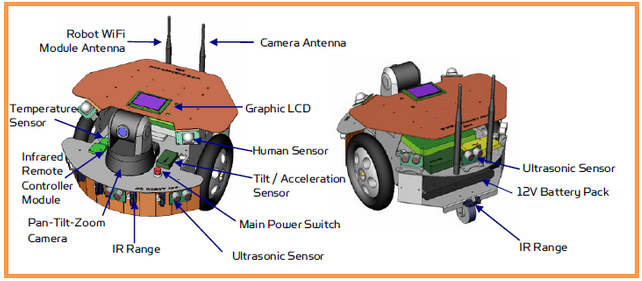
\includegraphics[scale=0.75]{images/X80SVPRobot}

\caption{\label{fig:X80SVP-Robot}X80SVP Robot \cite{:XSVPQuickStartGuide}}



\end{figure}


The Beagleboard XM was chosen as the computer for the X80SVP. Some
of the major advantages to this is that the Beagleboard has many peripheral
options, a 1 GHz CPU, a DSP, and it is very popular in the open source/ROS
communities. The initial plan accounted for the DSP being able to
process the Kinect vision data while the CPU handled the overhead
associated with ROS. The major components on the board are shown below
in Figure \ref{fig:Beagleboard's-Main-Components}.

%
\begin{figure}[H]
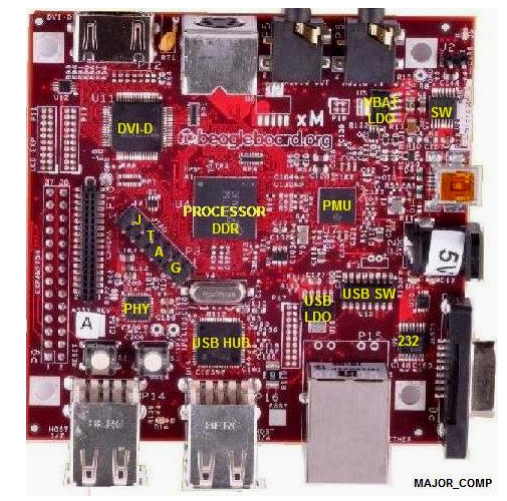
\includegraphics[scale=0.4]{images/beagleboardMajorComps}

\caption{\label{fig:Beagleboard's-Main-Components}Beagleboard's Main Components
\cite{:BeaglSysteReferManua}}

\end{figure}


A Kinect was used to generate maps of the robot's surroundings and
to allow the robot to navigate intelligently through his environment.
The OpenNI drivers for ROS, created by the makers of the Kinect, would
enable the Kinect to be used in this manner. One of the main concerns
with using the Kinect was the processing power that it would require.
The Kinect produces a message that is roughly 10 MB at a rate of 30
frames per second, this equates to the Kinect sending about 300 MB
of data each second. At first, it was expected that the DSP on the
Beagleboard would have been able to handle the Kinect\textquoteright{}s
processing; however, due to the overhead of ROS, the processing will
most likely have to be offloaded to a netbook. 


\section*{Technologies}

ROS is a framework that facilitates the construction and execution
of applications for robots. There are implementations of ROS in C++,
Python, Lisp, and Java. ROS executables are called nodes. ROS provides
a master node that oversees running nodes and a parameter server,
it also acts as the matchmaker for nodes and topics. ROS nodes communicate
over topics or services using ROS methods. Nodes publish messages
on topics which other nodes can subscribe to in order to receive the
information. The message's fields are described in a data file using
the yaml language which ROS converts into a file that the targeted
language can use, such as a header file in C++.

ROS also provides a hierarchy to group common elements. Nodes that
perform common functions are grouped into a package. Packages that
share a common purpose are grouped into stacks. Therefore, ROS's goal
is to build a complex system out of simple, single-purpose parts.

The rosjava stack is an implementation of ROS in Java; therefore,
rosjava nodes work with the rest of the nodes in ROS. In order for
rosjava nodes to communicate, ROS messages are converted to classes
and made into jar files; this allows for easy integration of message
data types into rosjava nodes.


\section*{Obstacle Avoidance Algorithm}

There are two ways to implement obstacle avoidance. One implementation
is motor fusion, which uses a direct correlation between sensor readings
and motor velocities. The second implementation, sensor fusion, uses
the sensor data to reconstruct the surroundings to produce motor commands.
For the X80SVP robot, obstacle avoidance was accomplished by a motor
fusion algorithm utilizing Braitenburg's aggression behavior.

Braitenburg behaviors are a form of synthetic psychology described
in Valentino Braitenberg\textquoteright{}s book\cite{braitenberg1986}.
These behaviors were thought experiments into how different emotions,
such as fear, aggression, and love, can provoke movement based on
sensor stimulation. Aggression behavior is caused by pairing the sensors
and motors on opposite sides through a non-decreasing function.

To implement aggression behavior for obstacle avoidance, modifications
to use a centered sensor were made to the algorithm presented in \cite{ran2005obsavothrbraaggbehmotfus}.
The algorithm computes both the linear and angular velocity for the
robot given the normalized sensor readings as shown in equations \ref{eq:translationalSpeed}
and \ref{eq:rotationalSpeed}. Accounting for the center sensor separately
allows the robot to avoid deadlock while in symmetric corners. The
value of the sensor increases as an obstacle gets farther away and
as the velocity becomes greater in that direction, providing a smooth
wandering movement that effectively avoids obstacles.

\begin{equation}
\alpha_{S}(t_{k})=\sum_{i\in L\cup R}w_{i}^{\alpha_{S}}\hat{r}_{i}^{S}(t_{k})\label{eq:translationalSpeed}\end{equation}


\begin{equation}
\beta_{S}(t_{k})=\sum_{i\in R}w_{i}^{\beta_{S}}\mathfrak{D}(\theta'_{i})\hat{r}_{i}^{S}(t_{k})-\sum_{i\in L}w_{i}^{\beta_{S}}\mathfrak{D}(\theta'_{i})\hat{r}_{i}^{S}(t_{k})\label{eq:rotationalSpeed}\end{equation}


$\alpha_{S}$ and $\beta_{S}$ are the normalized translational and
rotational speeds in the range {[}0,1{]} and {[}-1,1{]} respectivley.
$w_{i}^{\alpha_{S}}$ and $w_{i}^{\beta_{S}}$ are constant weights
corresponding to the $i^{th}$sensor defined in equations \ref{eq:translationalWeight}
and \ref{eq:rotationalWeight}. $\hat{r}_{i}^{S}(t_{k})$ is the current
normalized filtered range value of the $i^{th}$ sensor. $\mathfrak{D}(\theta'_{i})=90-|\theta_{i}|$
the angular distance. Where $\theta_{i}$ is angle from the x-axis
to the sensor assuming the x-axis lies on the axle and y-axis divides
the robot in half.

\begin{equation}
\mathit{w}_{i}^{\alpha_{S}}=k_{i}^{\alpha}e^{-\frac{\mathfrak{D}(\theta'_{i})^{2}}{2\sigma_{\alpha}^{2}}}\label{eq:translationalWeight}\end{equation}


\begin{equation}
\mathit{w}_{i}^{\beta_{S}}=k_{i}^{\beta}e^{-\frac{\mathfrak{D}(\theta'_{i})^{2}}{2\sigma_{\beta}^{2}}}\label{eq:rotationalWeight}\end{equation}


$k_{i}^{\alpha}$ and $k_{i}^{\beta}$ are normalizing constants so
that the speeds are normalized. $\sigma_{\alpha}^{2}$ and $\sigma_{\beta}^{2}$
are the variance chosen here to be 1400 and 350 respectively. 


\section*{Simulator Libraries}

The simulator uses a number of libraries to make the OpenGL API more
manageable. FreeGLUT is used to provide the basic windowing functions
for the GL application. GLU provides utility functions for computing
projection matrices, used to create the perspective camera views.
SOIL is used to provide texture-loading capabilities. The simulator
also interfaces directly with the Xorg APIs for some functions in
handling mouse and full-screen controls. A custom loader was written
to load DirectX format mesh files exported by Blender. This allows
environments as well as movable obstacles of completely arbitrary
design and complexity to be modelled quickly.


\part*{Design}

The design model favors modularity and simplicity to create a complex
system. The goal was to follow the subsumption control architecture
to create a robust and fault tolerant system. By following the model
view controller design pattern, the implementation is extensible.
The model is based on the ROS parameter server in which the model
of the robot and communication layout is stored. The view is the world
or the virtual world as created by the simulator. The controller classes
act to move the robot, changing the robot\textquoteright{}s view. 

%
\begin{figure}[H]
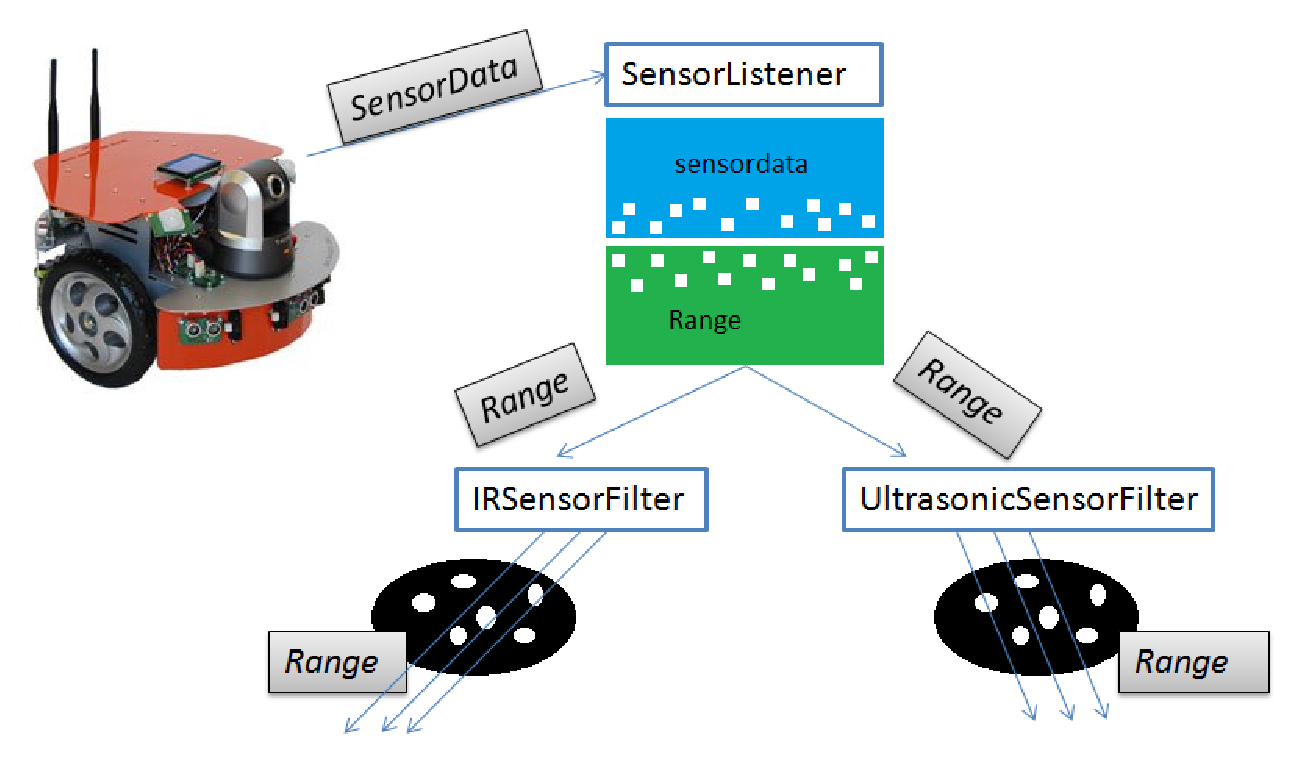
\includegraphics[scale=0.35]{images/SensorComm}\includegraphics[scale=0.45]{images/obstAvoid\lyxdot PNG}

\caption{\label{fig:Simplified-Design-and}Simplified Design and Communication
Model}



\end{figure}


The design is centered around the Converter and the RobotActor classes.
Converter and RobotActor are interchangeable bridges between the view
and the control, they publish the sensor data and send commands to
actuate the robot\textquoteright{}s motors. The SensorListener class
subscribes to the sensor messages published by a bridge class and
publishes converted sensor data in the ROS standard Range message
type. The SensorFilter classes filter the sensor data so that the
data is more useful and the BraitenburgAvoid class uses the filtered
sensor data to publish a MotorCommand message based on the Braitenburg
aggression behavior algorithm. The ObstacleAvoidance node publishes
a linear combination of the MotorCommand sent by the infrared and
ultrasonic based on BraitenburgAvoid nodes. Finally, the MotorController
acts as both an arbiter of motor commands and as a gateway back to
the bridge nodes. The full design diagram is in Appendix A.

The initial design of the simulator relied on existing code which
supported only one \textquotedblleft{}Player\textquotedblright{} with
one graphical view; this was adapted to support an arbitrary number
of \textquotedblleft{}Actors\textquotedblright{}, each with any number
of \textquotedblleft{}Sensors\textquotedblright{}. This was then used
to implement each of the ultrasonic and infrared sensors as well as
the graphical displays. Multiple actors allow the user to view the
environment from the perspective of the robot or from an independent
Camera actor, it also allows Obstacle actors to be positioned in real-time.
A diagram of the simulator appears in Appendix B.


\part*{Implementation}

The implementation of the design was completed in both C++ and Java.
C++ was used for the simulator and the serial communication between
the robot and Beagleboard while Java was used to implement the rest
of the design.

The serial library used the PMS5005 protocol which allows any processor,
DSP, or PC to control the robot through the Universal Asynchronous
Receiver/Transmitter (UART) communication interface. The basic packet
outline, shown in Figure \ref{fig:Packet-format-for}, handles both
the sensor and motor data transmission. The library that implements
this interacts with ROS by subscribing to motor controls and publishing
sensor data. Using this packet structure, a large amount of information
can be processed every tick.

%
\begin{figure}[H]
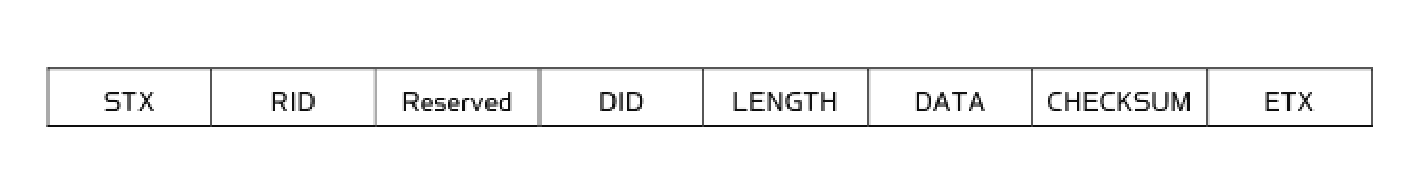
\includegraphics[scale=0.5]{images/packet}

\caption{\label{fig:Packet-format-for}Packet format for serial library}

\end{figure}


The sensor and motor data from the packet structure were not ideal
for our purposes and needed to be converted to useful formats. The
data for the sensors needed to be handled differently for each type
of sensor. The ultrasonic sensors were the most straightforward since
the control board returned the distance in the range of 0 - 255 cm,
which is already in the correct units for the message. The infrared
sensors needed to be converted since they return a non-linear voltage
value corresponding to a range of 10 - 80 cm. The voltage output with
respect to distance is shown in Figure \ref{fig:Infrared-sensor-voltage}.
This voltage output needed to be linearized using an interpolation
equation \cite{:LinearizingSharpRangerData}. The result of such an
equation with respect to Analog/Digital Converter (ADC) values is
shown in Figure \ref{fig:Linear-interpolation-of}. After testing
the human sensors, it was decided that these will not be used at this
point due to unreliable results.

%
\begin{figure}[H]
%
\begin{minipage}[t]{0.45\columnwidth}%
\begin{center}
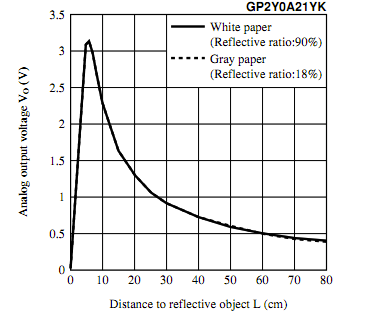
\includegraphics[scale=0.3]{images/voltageOutput}
\par\end{center}

\caption{\label{fig:Infrared-sensor-voltage}Infrared sensor voltage output
\cite{:SharpGPYAY} values \cite{:LinearizingSharpRangerData}}
%
\end{minipage}\hfill{}%
\begin{minipage}[t]{0.45\columnwidth}%
\begin{center}
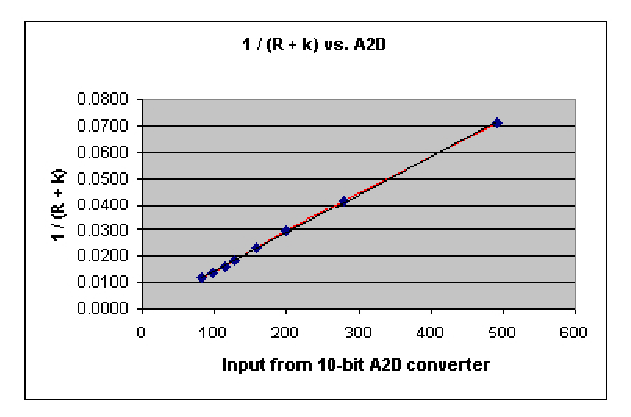
\includegraphics[scale=0.3]{images/ADCValues}
\par\end{center}

\caption{\label{fig:Linear-interpolation-of}Linear interpolation of Voltage
with respect to ADC}
%
\end{minipage}
\end{figure}


Once the serial library and sensor conversions were implemented on
a desktop system, the next step was to achieve this functionality
on the Beagleboard. The Beagleboard was loaded with Ubuntu 11.10 since
this OS works best with ROS. Some of the configuration scripts for
ROS require Internet access so a wireless internet connection was
part of the Beagleboard setup. ROS was compiled from source on the
Beagleboard because cross compiling is not recommended for ROS yet.
After configuring the installation, it quickly became apparent that
the overhead associated with ROS was more than expected. At the moment,
the Beagleboard is unable to support ROS at 10 Hz and further testing
will conclude whether this can be fixed or not.

The obstacle avoidance algorithm produces linear and angular velocity
values, but the robot requires left and right wheel velocities. Using
the differential drive kinematics equations \ref{eq:LeftVelocity}
and \ref{eq:RightVelocity}, the conversion is possible. Note that
$\alpha_{S}(t_{k})$ and $\beta_{S}(t_{k})$ are normalized linear
and angular velocities and d is the wheel base of the robot.

\begin{equation}
V_{L}=\frac{2\alpha_{S}(t_{k})+d\beta_{S}(t_{k})}{2}\label{eq:LeftVelocity}\end{equation}


\begin{equation}
V_{R}=V_{L}-d\beta_{S}(t_{k})\label{eq:RightVelocity}\end{equation}


Ultrasonic sensors were used to provide obstacle avoidance, however
the sensors can overestimate the distance to a flat wall due to specular
reflection. These readings can be improved by applying an incremental
filter (Equation \ref{eq:USFilter}) as described in \cite{ran2005obsavothrbraaggbehmotfus}.
The filter works by acting as a short term memory to ensure that a
current reading of free space is correct based on the previous range. 

\begin{equation}
\tilde{r_{i}}(t_{k})=\begin{cases}
r_{i}^{s}(t_{k}) & \textrm{if }r_{i}^{s}(t_{k})<r_{nr}^{s}\\
Min\{\tilde{r_{i}}(t_{k-1})+r_{\triangle},r_{nr}^{s} & \textrm{if }r_{i}^{s}(t_{k})=r_{nr}^{s}\end{cases}\label{eq:USFilter}\end{equation}


$r_{nr}^{s}$is the max range of the sensor, $r_{i}^{s}(t_{k})$ is
the current range measurement, $\tilde{r_{i}}(t_{k})$ is the current
filtered range value and $\tilde{r_{i}}(t_{k-1})$ is the previous
filtered value.

One issue of using rosjava was the overhead of creating new nodes,
since each new node started a new JVM process. After implementing
the design of the rosjava nodes, rosjava released documentation detailing
how using a NodeRunner object can start the nodes as threads rather
than as new processes. This significantly reduced the memory overhead
and launch time of the rosjava nodes.

RGBDSLAM was selected as the main algorithm to implement mapping.
In order to take advantage of RGBDSLAM, the entire project had to
be downgraded from using ROS Electric to ROS Diamondback and from
using Ubuntu 11.04 to Ubuntu 10.10. RGBDSLAM allows a point cloud
of the environment to be created from the Kinect data as seen in Figure
\ref{fig:RGBD-point-cloud}. Once a point cloud was generated, it
could be converted to an OctoMap as seen in Figure \ref{fig:Octomap},
a 3D occupancy grid map that is developed from an octree. The OctoMap
is then sent to the 3D navigation algorithm so that the robot can
utilize the map.

%
\begin{figure}[H]
%
\begin{minipage}[t]{0.45\columnwidth}%
\begin{center}
\includegraphics[scale=0.3]{\string"images/rgbdslam point cloud fig 1\string".eps}
\par\end{center}

\caption{\label{fig:RGBD-point-cloud}RGBD point cloud}
%
\end{minipage}\hfill{}%
\begin{minipage}[t]{0.45\columnwidth}%
\includegraphics[scale=0.3]{\string"images/octomap fig 2\string".eps}

\caption{\label{fig:Octomap}Octomap}
%
\end{minipage}
\end{figure}


The original goal was to have the robot using a static OctoMap to
navigate his environment, and eventually implement dynamic mapping
so the robot would have been able to map his environment while he
wandered. Due to issues with ROS running in a timely matter on the
Beagleboard, it is unsure as to whether the OctoMaps will be usable.
At this point, a sign language feature may be replacing the OctoMaps,
but that will be more-so determined in the final paper.

One of the initial challenges encountered in writing the simulator
was that the position of the robot was represented as a point on an
X-Y plane, but the input coming in from ROS would be in the form of
differential wheel movement commands. Finding the necessary equations
proved to be a challenge. It was also difficult to test initially
since the ROS interface had not yet been implemented to a working
degree. Some revisions and corrections had to be done once it was
possible to send specific commands from ROS and to observe whether
the resultant location of the robot in the simulation was correct.

%
\begin{figure}[H]
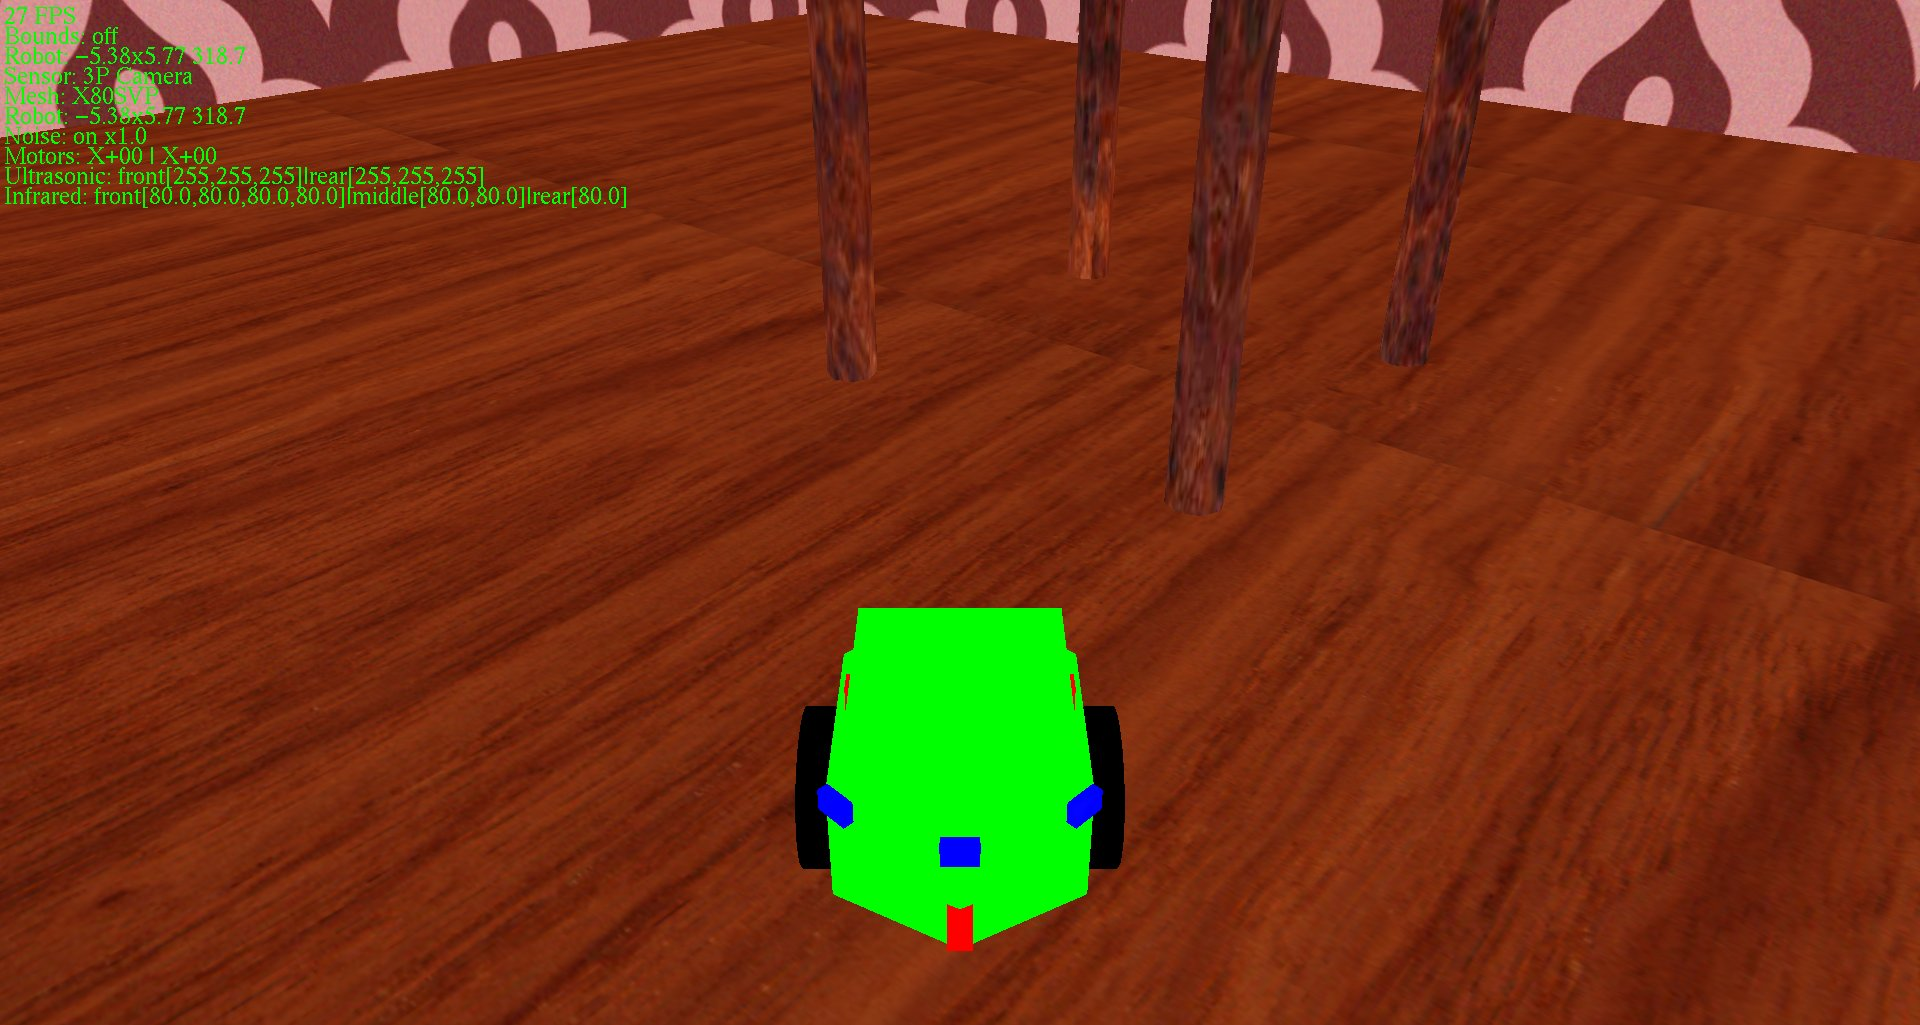
\includegraphics[scale=0.2]{images/3rdperson}

\caption{Simulator in third person view}

\end{figure}


There were some problems to overcome in terms of speed and optimization.
One of these problems was in computing a linear representation of
the depth map because GL uses a logarithmic representation when rendering,
but the one provided by the Kinect is linear. The initial implementation
of this conversion required doing up to two million floating-point
logarithm operations per frame. This was improved significantly by
making the simulator initially render at the Kinect hardware's resolution,
then scaling it to fit the actual size of the visualization window.
Performing the conversion in this manner provided a nearly seven-fold
reduction in the number of required operations when running in fullscreen
mode.

%
\begin{figure}[H]
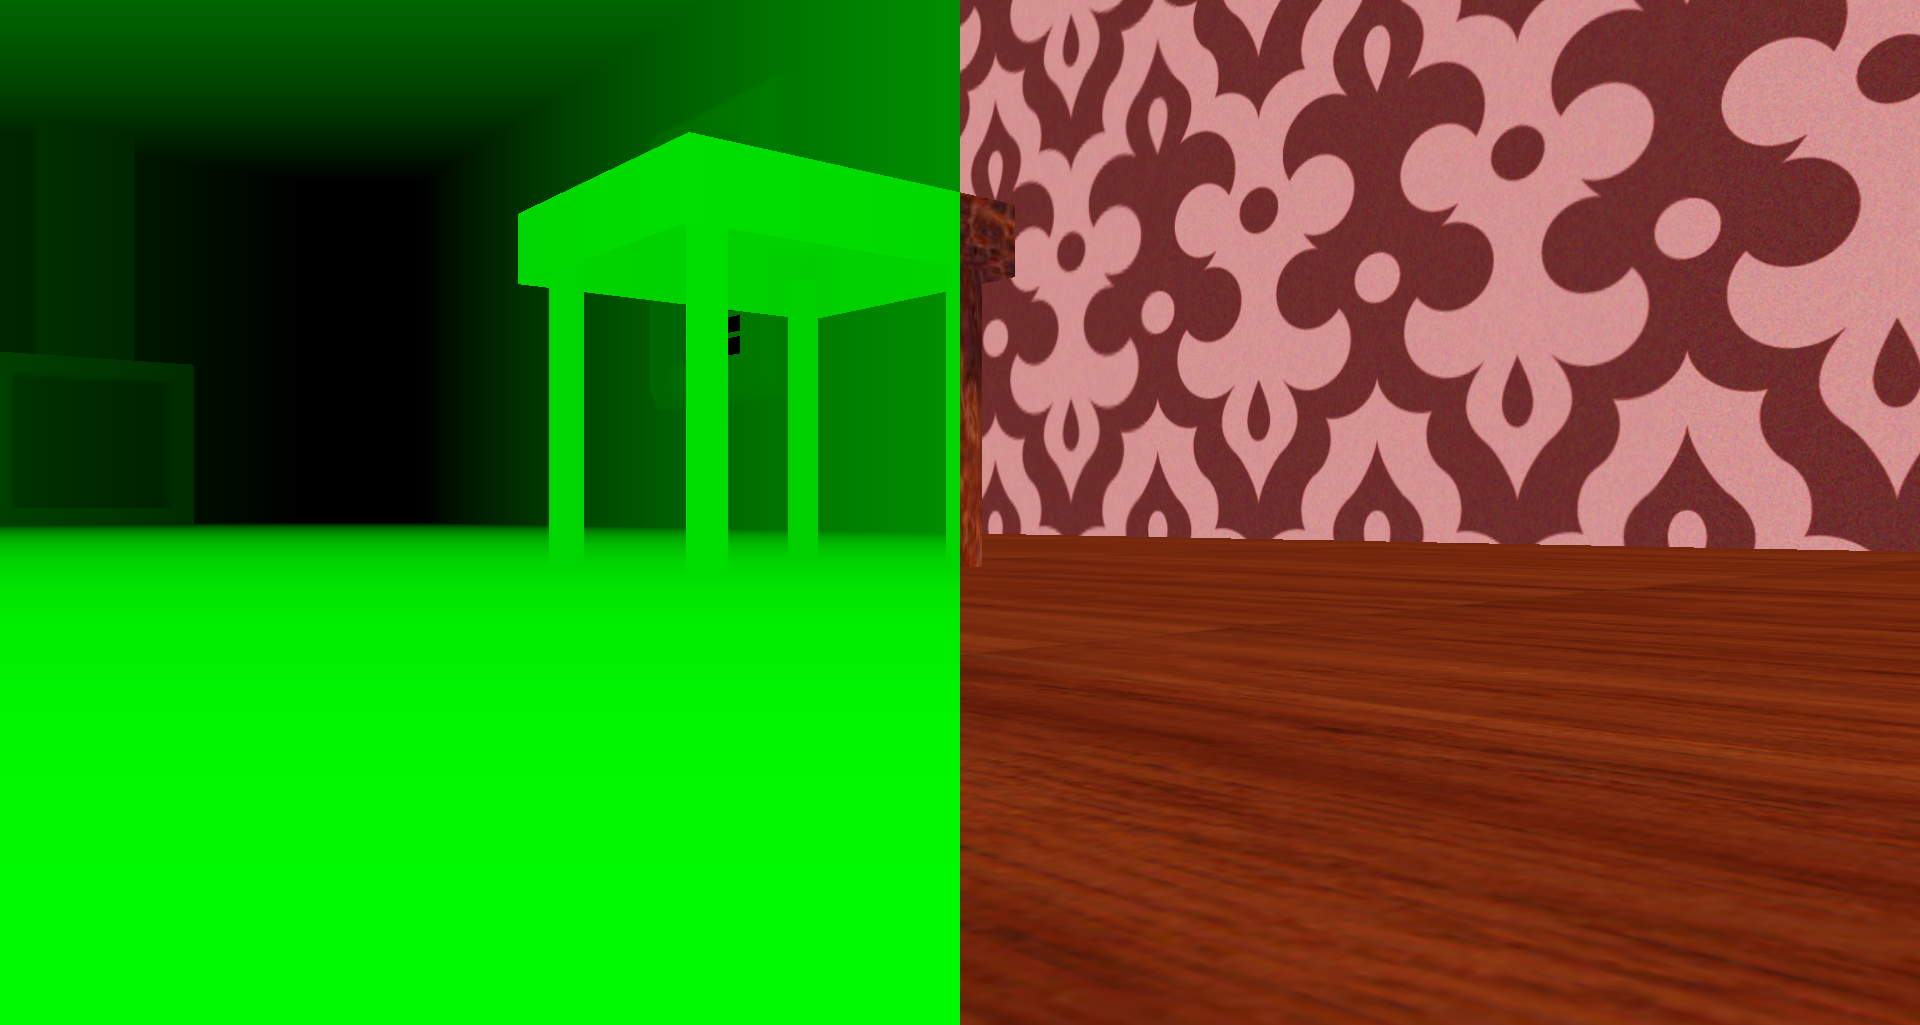
\includegraphics[scale=0.2]{images/depthmap}

\caption{Simulated Kinect depth map}



\end{figure}


There were also some modifications in what is rendered during each
pass. The simulator visualization targets a frame rate of 60 fps,
but was unable to attain that rate on the workstation. Since the Sensing/Motion
Controller on the actual robot only functions at 10 Hz, it is only
necessary to broadcast data to ROS at that rate; thus, the sensor
rendering passes could be skipped on 5/6ths of the frames, saving
processing resources and boosting frame rate.


\part*{Future Work}

In the future, there are plans to implement features such as gesture
recognition, a multi-agent system, and unit testing for the simulator.

Gesture recognition is one of the more immediate future plans for
the robot. A ROS stack called hand\_interaction, created by the Massachusetts
Institute of Technology, appears to be the best option for implementing
this feature. Using hand\_interaction, the location of the hands can
be determined. As a gesture is made, the movement of the hands will
be tracked and then the robot can react accordingly. At this point,
it is unknown as to whether the gestures should be hard-coded into
the robot or if the robot should learn these gestures manually. The
most beneficial of these options will be determined and mentioned
in the final paper. 

The system could be extended by adding TurtleBots to create a multi-agent
system. Capture the flag could be a way to explore algorithms involved
in multi-agent systems. However, due to the limited processing power
of the Beagleboard, there would be considerable challenges implementing
efficient navigation, SLAM, and learning algorithms. One solution
would be to use a remote computer to perform these features.

Another way the system could be extended is by using the Kinect for
facial and object recognition. This would allow for high level behavior
and learning rather than the current reactive-based system; however,
the processing capabilities of an on-board computer may be overwhelmed.

A future system could also utilize rosjava\textquoteright{}s ability
to operate on Android to provide a user with the ability to teleoperate
the robot or provide the robot access to the cloud.

A way to implement unit testing in the simulator may be useful. This
would allow some of the previous problems encountered, such as inaccuracies
in the wheel movement equations and rendering pipeline issues causing
inaccurate sensor outputs, to be tracked down more quickly. Implementing
this may be difficult, as the correct values would have to be computed
manually by some other reliable method, and one of the primary motives
for developing the simulator was to not have to do these tedious calculations
manually.


\part*{Appendix}


\section*{Section A\label{sec:Appendix-A}}

Updated design model shows how messages and nodes relate.

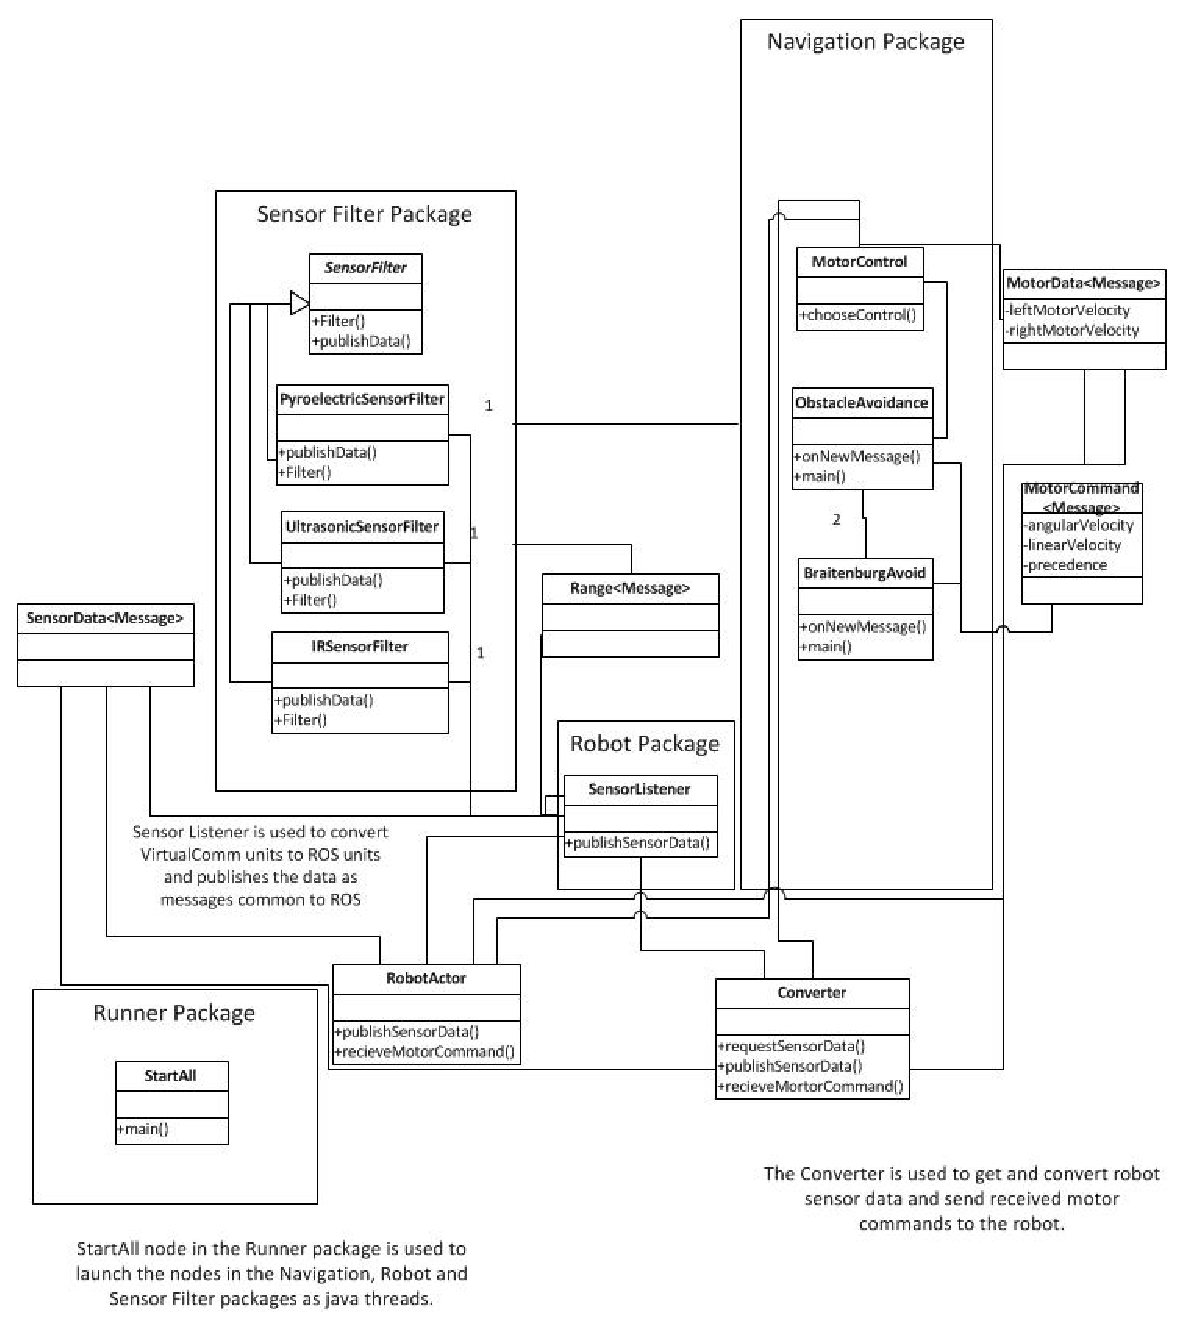
\includegraphics[scale=0.65]{images/DesignModel}


\section*{Section B\label{sec:Appendix-B}}

The User can select to control any Actor's position. The specific
sensor the CameraView is rendered from can also be selected. Data
from ROS is also used to control the RobotActor's position and the
Sensors are output back to ROS.

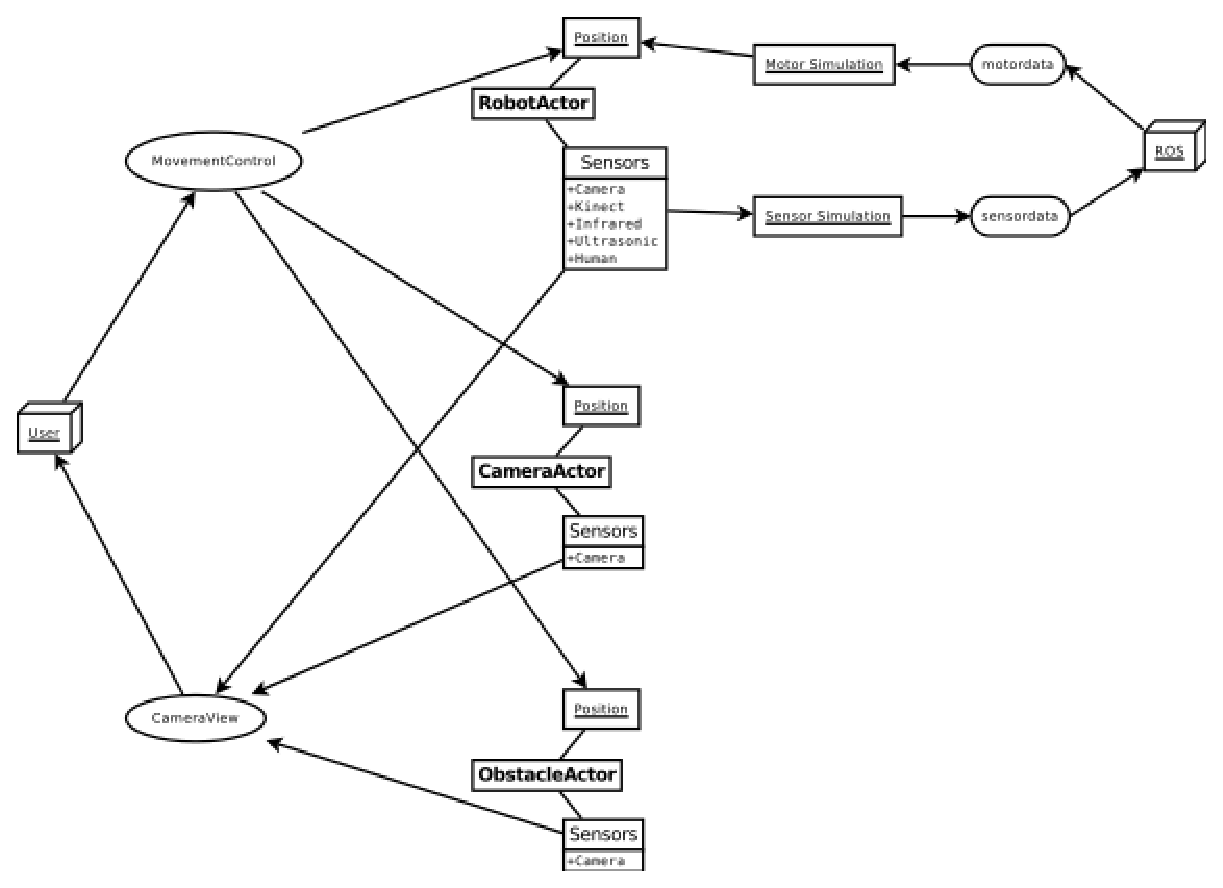
\includegraphics[scale=0.65]{images/Sim}

\bibliographystyle{plain}
\nocite{*}
\bibliography{bibliography}

\end{document}
